% Software License Agreement
%
% Author    Chris Bogdon <cbogdon@clearpathrobotics.com>
% Copyright (c) 2015, Clearpath Robotics, Inc., All rights reserved.
%
% Redistribution and use in source and binary forms, with or without modification, is
% not permitted without the express permission of Clearpath Robotics.


\documentclass[]{clearpath-latex/clearpath-manual}
\graphicspath{{gen/}}
\usepackage{multirow}
\usepackage{gensymb}
\usepackage{dcolumn}
\usepackage{colortbl}
\usepackage{array}
\usepackage{hyperref}

\begin{document}

\manualcover{cover-page.pdf}
\tableofcontents

\section{Introduction}
Clearpath Robotics Ridgeback is a sturdy omnidirectional platform designed to move manipulators and other heavy payloads with ease. This guide contains information about the setup, operation, and maintenance of your Ridgeback.

\subsection{What's Included}

Included with each Ridgeback are the following:

\begin{itemize}[nolistsep]
	\item 1x Ridgeback 
	\item 1x Battery Pack
	\item 1x Universal battery charger
	\item 1x Sony Bluetooth controller
	\item 1x Ridgeback User Manual
	\item 1x Onboard Mini ITX Computer with ROS Platform
	\item 1x Hokuyo UST-10LX forward facing LIDAR
\end{itemize}

\subsection{Expansions}

To expand the capabilities of Ridgeback, consider the following integrated packages offered by Clearpath Robotics:

\subsubsection{Baxter Package}

The Baxter Package includes an adjustable podium mount, power system tie-ins and communication for Baxter, enabling the robot to be integrated in under 30 minutes. Easily coordinate behaviours between Ridgeback and Baxter with full ROS, Gazebo Physics Simulator, RViz and MoveIT! Motion planner support.

\textbf{Included Accessories:}
\begin{itemize}[nolistsep]
	\item Baxter Mounting Podium
	\item 120/240V VAC power inverter
\end{itemize}

\subsubsection{UR5 Package:}

The UR5 Package includes mechanical mounting, integrated UR5 controller, power and communications for the Universal Robotics UR5 robot arm. It also includes a Robotiq 3-Finger gripper and a force torque sensor. Easily coordinate behaviours between Ridgeback and UR5 with full ROS, Gazebo Physics Simulator, RViz and MoveIT! Motion planner support.

\textbf{UR5 Packages}

\textbf{Included Accessories:}

\begin{itemize}[nolistsep]
	\item BUR5 robot arm
	\item 3 Finger 85 Robotiq gripper
	\item Robotiq FT 150 force-torque sensor
	\item BumbleBee stereo camera
	\item FLIR PTU D46-17 pan-tilt unit
\end{itemize}

\subsection{Hardware Overview}

\begin{figure}[h]
  \centering
  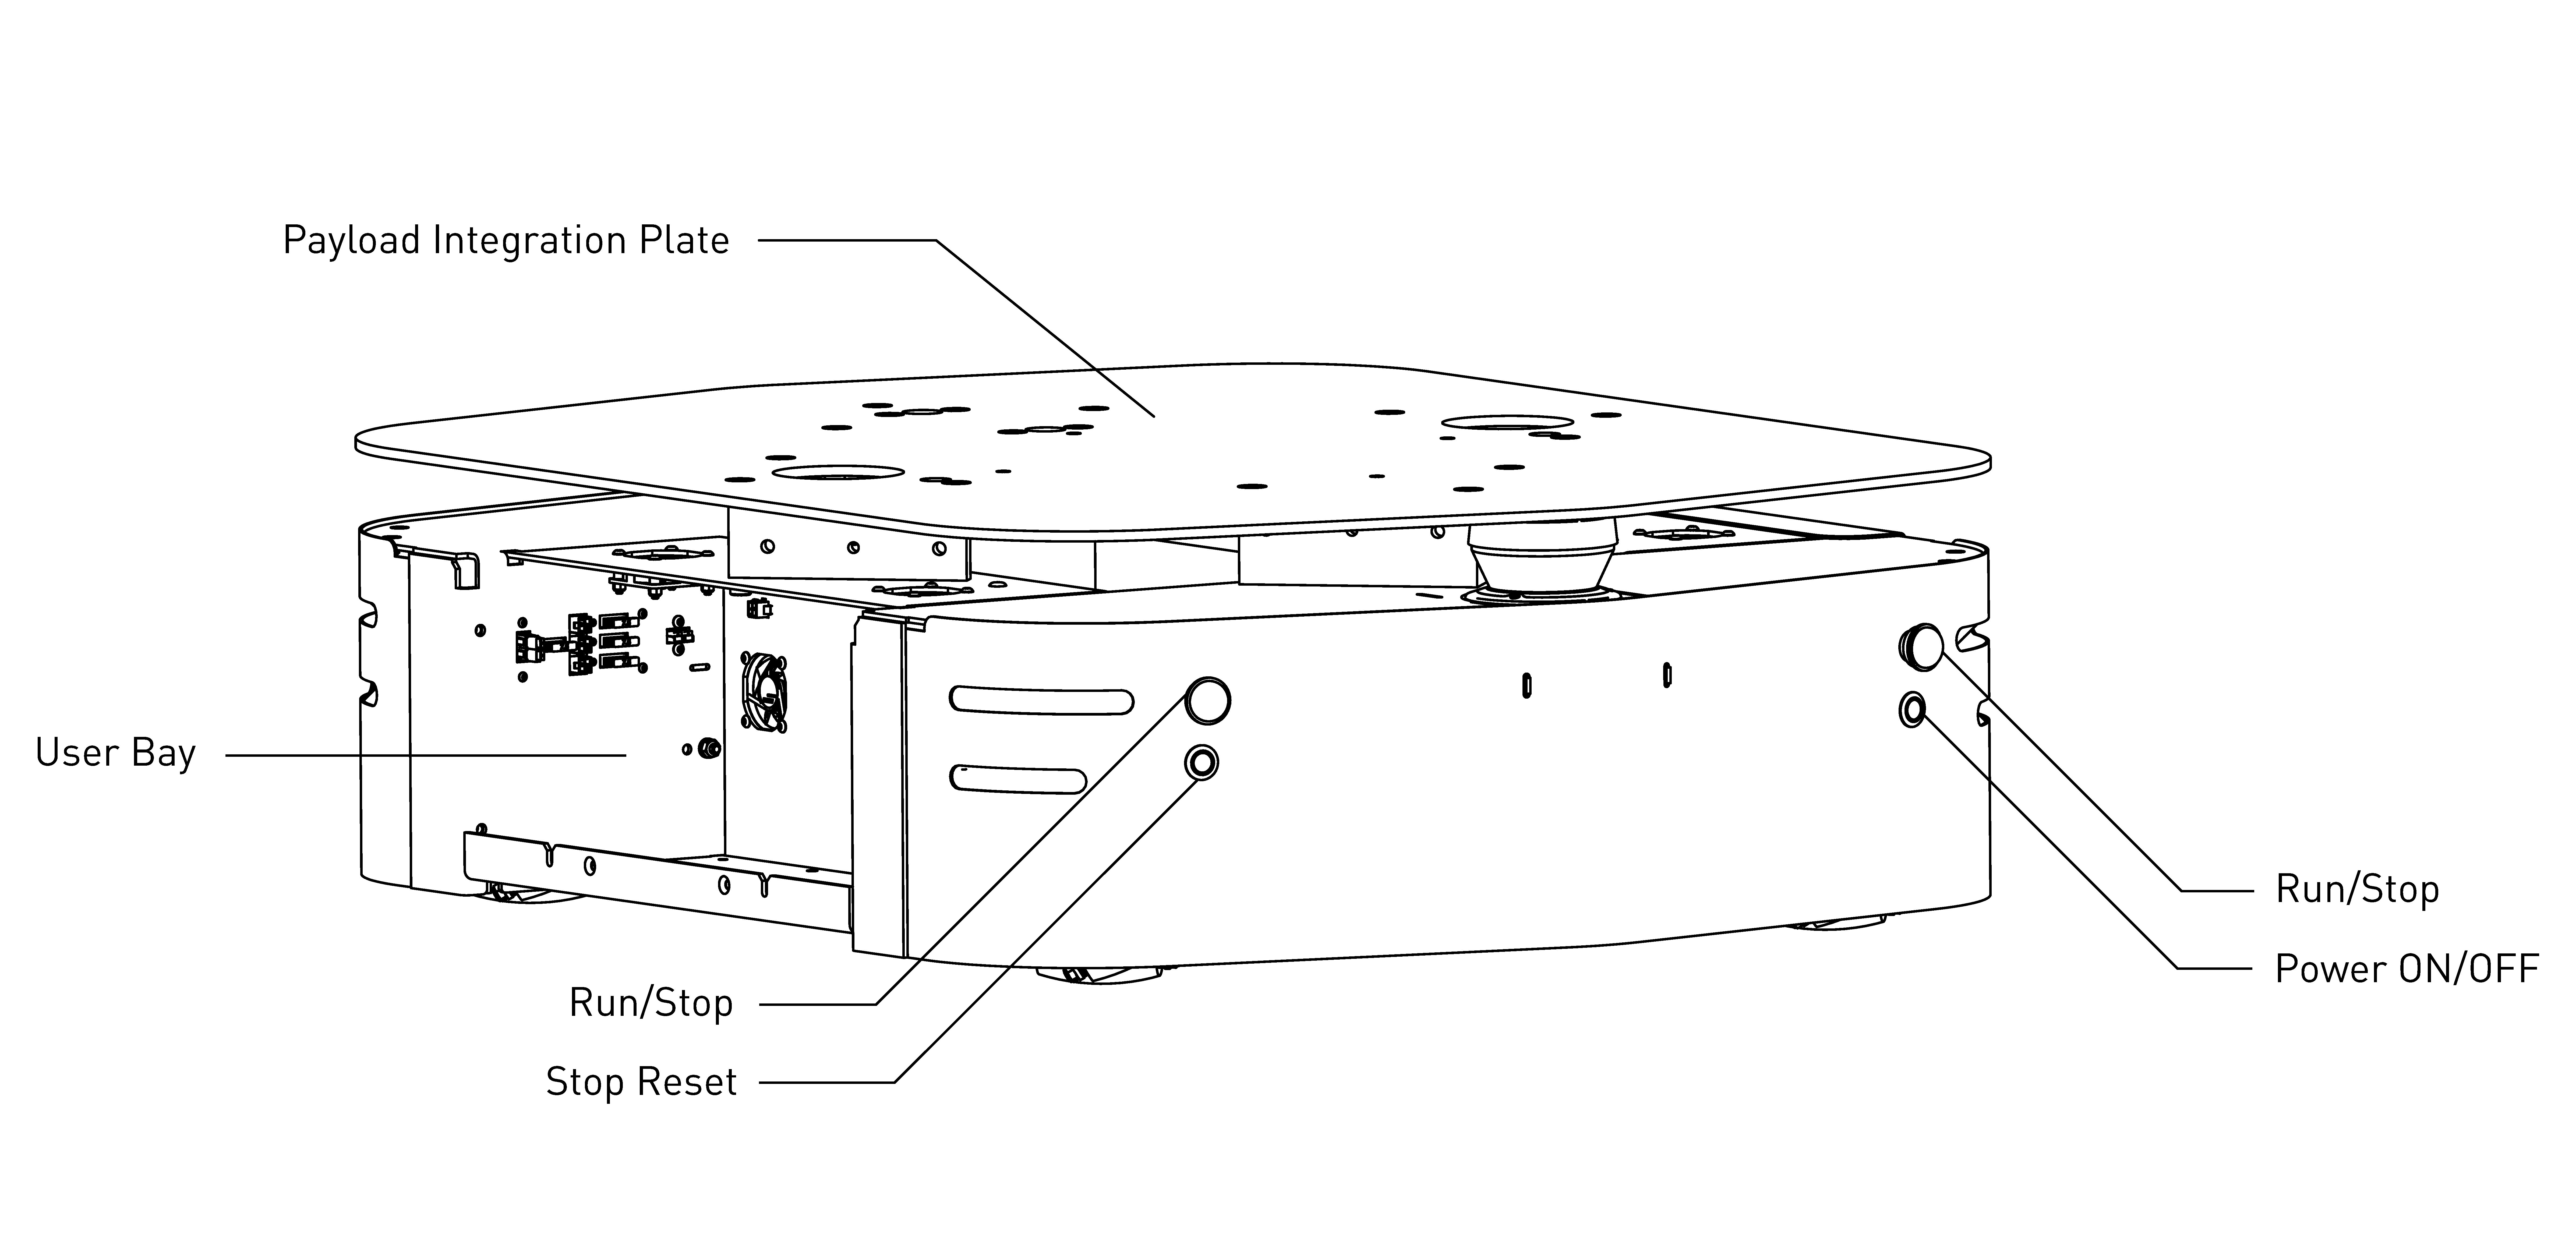
\includegraphics[width=1\linewidth]{Ridgeback_Rear_Drawing_Labeled.pdf}
  \caption{Ridgeback Hardware Overview}
  \label{ridgeback_overview}
\end{figure}

\subsubsection{Rear Buttons}

There are four push buttons located on the back of the Ridgeback: Stop, Stop Reset and Power ON/OFF.   Each button is described in \autoref{rearbuttons}. 

\bgroup
\def\arraystretch{1.2}%
\begin{table}[h]
	\centering
	\begin{tabular}{>{\columncolor{lightgrey}}>{\raggedright}m{.25\textwidth} p{.75\textwidth}} \hline 

	Power ON/OFF & Turns on/off the Ridgeback. \\ \hline

	Stop (x2) & Stops the robot.  Intended for use in emergency situtions.  To release, twist the button in counter-clockwise direction.  \\ \hline	
	
	Stop Reset & Allows Ridgeback to run again after it has been stopped via Stop button.    \\ \hline	
	
	\end{tabular}
\newline
\caption{Ridgeback Rear Buttons}
\label{rearbuttons}
\end{table}
\egroup


\subsubsection{User Bay}

The User Bay provides access to the User Power electrical panel, USB and Ethernet ports, and additional space for stowing user equipment.  The electrical panel can be used to power your payload structures.   The Ethernet and USB ports can be used to connect your payload structures to the onboard PC.  

For more information on electrical integration, please see Electrical Integration on page \pageref{electrical}.


\subsubsection{Payload Integration Plate}

The Payload Integration Plate provides a robust foundation for mounting payload stuctures such as Baxter, UR5/UR10 manipulation arms, or any other combination of sensors and manipulators.   For more information and guidance on mounting payload structures ontop of Ridgeback, plage refer to Mechanical Mounting on page \pageref{mechanical}.



\subsection{System Architecture}

\begin{figure}[!htb]
  \centering
  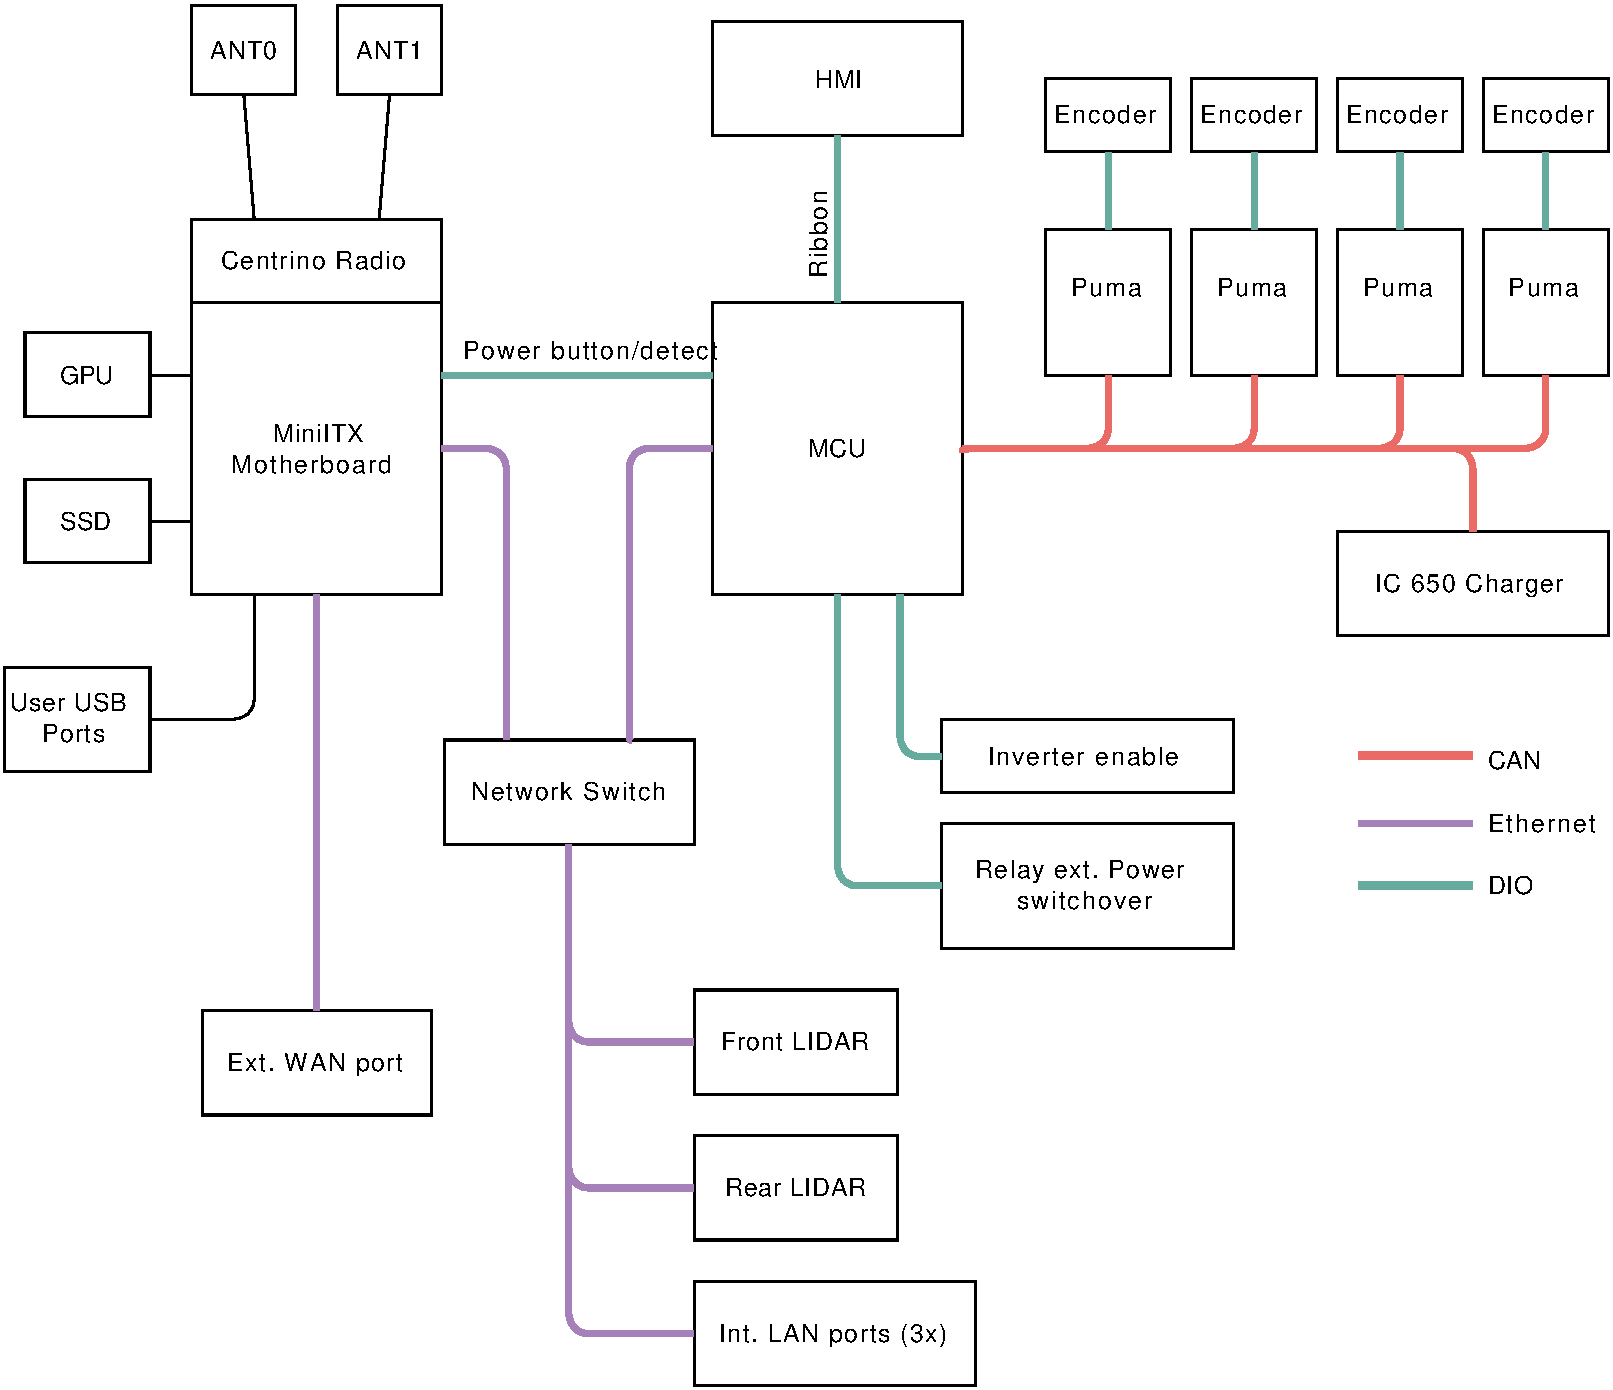
\includegraphics[width=0.75\linewidth]{ridgeback-logic-conn.pdf}
  \caption{System Architecture}
  \label{systemarchitecture}
\end{figure}

\clearpage

\subsection{Technical Specifications}

Key specifications of Ridgeback are shown in \autoref{systemspecs}.

\bgroup
\def\arraystretch{1.2}%
\begin{table}[h]
	\centering
	\begin{tabular}{>{\columncolor{lightgrey}}>{\raggedright}m{.30\textwidth} p{.70\textwidth}} \hline 

	External Dimensions (L x W x H) & 932 x 793 x 298 mm   (36.7 x 31.1 x 11.7 in) \\ \hline
	Weight & 125 kg (275 Ilbs) \\ \hline
	Obstacle Clearance & 18 mm (0.7 in) \\ \hline
	Max Payload  &  100kg (220 lbs)  \\ \hline
	Max Speed  &  1.1 m/s (3.6 ft/s) \\ \hline
	Drive Configuration &  4 Independently driven omni-directional wheels \\ \hline
	Operating Environment  &  Indoor \\ \hline
	Battery Chemistry & Marine Grade AGM Sealed Lead Acid \\ \hline
	Capacity &  24 V 100 Ah \\ \hline
	Operating Time & 4 hrs typical, 8 Hours max \\ \hline
	Charge Time &  5 Hours approx \\ \hline
	User Power & 5 V, 12 V, 24 VDC (fused at 10A each), option 120 VAC \\ \hline
	Drive Power & 200 W peak, 800 W continuous \\ \hline
	Control Modes & Kinematic control (forward, sideways, rotation), individual wheel velocities \\ \hline
	Feedback & Battery, gyroscope and accelerometer \\ \hline
	Communication &  Ethernet, USB 3.0, RS 232 \\ \hline
	Drivers and APIs  &  ROS Indigo, Gazebo, Navigation Support, MoveIt! \\ \hline
		
	\end{tabular}
\newline
\caption{Ridgeback System Specifications}
\label{systemspecs}
\end{table}
\egroup

\subsection{Safety Considerations}

\subsubsection{General Warnings}

Ridgeback is a rugged and high-performance vehicle. For the safety of yourself and others, always conduct initial experiments and software development with the vehicle raised off the ground. Place a wooden crate, a set of sawhorses, a sturdy storage tub, or any other solid flat structure having a height greater than 6 inches under Ridgeback to keep the wheels clear of the ground (“up on blocks”).

When starting out, favor slower wheel speeds. Ridgeback's control loops can accurately maintain velocities as low as 0.1 m/s. Operating at such speeds will give you more time to react if things don’t go quite as you expect.

\subsubsection{Stop Buttons}

Two red Stop buttons are located on the back of Ridgeback. Power supply to Ridgeback's motor drivers is enabled by a normally-open relay, which is closed in series with the stop switch. When in Stop mode the Ridgeback will not drive. The commands received during stop are not buffered; Ridgeback will always act on the latest commands received. This means that if the commands are stopped before the Stop button is released, the Ridgeback will not move. If the commands are continued, Ridgeback will move at the speed commanded once the Stop is released.

Always ensure the Stop button is accessible at all times. Avoid mounting payloads that extend over the rear of Ridgeback and would occlude the Stop buttons.

\subsubsection{Electrical System}

Ridgeback is powered by two lead-acid (PbSO4) deep-cycle AGM batteries, similar to the type found in electric wheelchairs, golf carts, and other vehicles. Ridgeback's battery is capable of delivering 2000W. This gives Ridgeback motors their great performance, however, it is also enough power to cause severe bodily harm. Always use caution when operating Ridgeback to avoid personal injury or property damange.  To ensure saftey, please observe the following precautions:

\begin{itemize}[nolistsep]
	\item Do not tamper with the plug attached to the battery.
	\item Do not tamper with the fuse panel, except to check and change the fuses, and to connect and disconnect the 	battery plug.
	\item Always replace fuses with the same type and rating to ensure continued protection against risk of fires
	\item Always disconnect the battery before performing maintenance on the robot
	\item Do not lay tools or other objects on top of the battery   
	\item Do not move the robot while charging the battery
	\item Charge the battery only with the charger provided by Clearpath Robotics
	\item Please dispose of the batteries properly, or return the battery to Clearpath Robotics to do so
\end{itemize}

\subsubsection{Lifting and Transport}

\begin{itemize}[nolistsep]
	\item Ensure that Ridgeback's Stop button is engaged when transporting short distances and powered off when transporting longer distances
	\item Do not push the robot at more than 0.5 m/s (1.6 ft/s) or damage to the motor controls may occur
\end{itemize}

\subsubsection{Performance Recommendations}

Included in Ridgeback are native software checks and limits to protect the vehicle. However, it is recommended to monitor the system’s status during usage with \lstinline{/diagnostics/rqt_robot_moitor}.  

\begin{figure}[!htb]
  \centering
  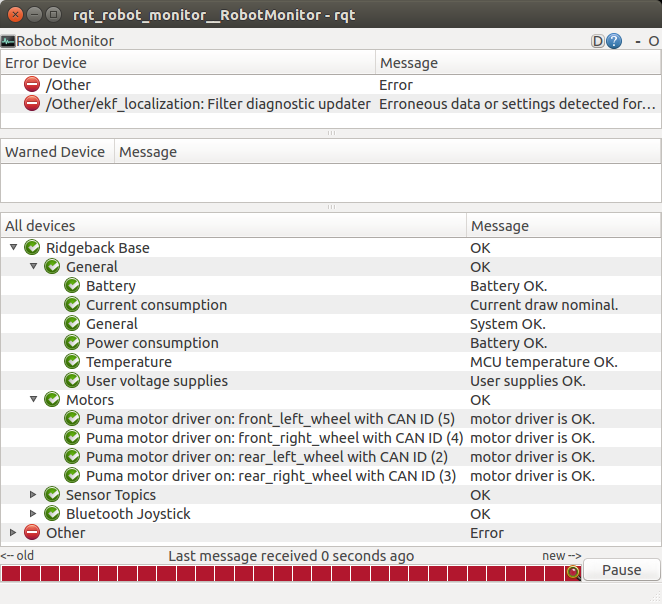
\includegraphics[width=0.75\linewidth]{rqt_robot_monitor.png}
  \caption{Robot Monitor}
  \label{robotmonitor}
\end{figure}



\section{Getting Started}

The first step is to power up your Ridgeback and have some fun driving it around! If you’ve just unpacked Ridgeback
from its shipment packaging, you’ll need to open it up and connect the battery.

Press the power button on the back of the Ridgeback. The LEDs should show a test pattern, after which you will
wait about 30 seconds for the internal PC to finish booting up.

Press the PS/P3 button on the Sony Bluetooth controller to sync the controller to Ridgeback. Once the small red
LED on the controller goes solid, you’re paired and ready to drive. Hold the L2 trigger button, and push the
thumbstick forward. For full speed mode, switch to the L1 trigger.

If you’re not seeing any action, check Contact on \autoref{contact} to get in touch with support.

\subsection{Wireless Access}

To get Ridgeback connected to your local wifi, you must first access the internal computer using a wired connection.
Open the User Bay, and connect to one of the the network ports with a standard
ethernet cable. Now, set your laptop’s ethernet port to a static IP such as \lstinline{192.168.1.51}, and connect via SSH
to \lstinline{administrator@192.168.1.1}. The default password is \lstinline{clearpath}.

Once connected via wire, execute \lstinline{wicd-curses} to enter the text/curses UI to the wireless interface configuration daemon (WICD). Within the text UI, you can configure which wireless network you’d like Ridgeback to connect to upon system startup.

When the wireless link is established, remove the network cable, re-establish your SSH session over wireless,
and close the Ridgeback User Bay.

\subsection{Remote ROS Connectivity}

Now that Ridgeback is on the wireless, you can access it via SSH or as a remote ROS master. Note that in
the default configuration, the background job running on Ridgeback launches with the \lstinline{robot_upstart} package,
which is configured to set the ROS\_IP environment variable to the static IP of the em1 ethernet port, by default
\lstinline{192.168.1.1}.

What this means is that in order for a workstation to communicate with Ridgeback over wireless, you may need to
change one of three things:

1. If you’re confident that Ridgeback will be operated only where it is connected to wifi, you could set
\lstinline{robot_upstart} to start the background ROS job only once wifi connects. To change this, run:

\begin{lstlisting} 
rosrun robot_upstart install ridgeback_base/launch/base.launch \
--job ros --interface wlan0
\end{lstlisting}


2. If you’re confident that your network will resolve hostnames correctly, you could change the generated
ROS start script (in \lstinline{/usr/sbin/ros-start}) to set the \lstinline{ROS_HOSTNAME} env var rather than \lstinline{ROS_IP}.

3. Finally, you can add a static route to your workstation which will route requests from 192.168.1.1 to
Ridgeback's real wireless IP on your network. An example of this configuration:

\begin{lstlisting} 
sudo apt-get install ros-indigo -robot-upstart
export ROS_MASTER_URI=http://192.168.1.1:11311
export ROS_IP=$(rosrun robot_upstart getifip wlan0)
sudo route add -net 192.168.1.1 netmask 255.255.255.255 gw $ROS_IP
\end{lstlisting}

These commands would be executed on your own machine.

Please contact Clearpath Support if guidance is required in selecting and executing a remote access strategy.
For more general details on how ROS works over TCP with multiple machines, please see:

\url{http://wiki.ros.org/ROS/Tutorials/MultipleMachines.}

For help troubleshooting a multiple machines connectivity issue, see:

\url{http://wiki.ros.org/ROS/NetworkSetup}


\subsection{Visualizing Ridgeback}

To command or observe Ridgeback from your desktop computer, first set up a basic ROS installation.  See the following page for details:

http://wiki.ros.org/indigo/Installation/Ubuntu

When your ROS install is set up, install the Ridgeback desktop packages:

\begin{lstlisting}
sudo apt-get install ros-indigo -ridgeback -desktop
\end{lstlisting}

Once your remote access to Ridgeback's ROS master is configured, you can launch rviz, the standard ROS robot visualization tool:

\begin{lstlisting}
roslaunch ridgeback_viz view_robot.launch
\end{lstlisting}

From within rviz, you can use interactive markets to drive Ridgeback, you can visulize its published localization estimate, and you can visualize any attached sensors which have been added to its robot description XML (URDF).  

Additionally from your desktop, you can launch the standard RQT Robot Monitor, which watches the diagnoztic output from Ridgeback's self-monitoring capabilities:

\begin{lstlisting}
rosrun rqt_robot_monitor rqt_robot_monitor
\end{lstlisting}

\section{Charging and Battery Maintenance}

Ridgeback uses two 8A31DTM Group-31 lead-acid (PbSO4) deep-cycle AGM batteries mounted low in the chassis. They provide an output of 24Vdc (nominal) and 100Ah of capacity and also serve as ballast to help keep the centre of gravity of the robot low, even with payloads mounted atop it.

Ridgeback has an internal charger. All that is required to charge Ridgeback is to open the User Bay access panel, locate the charger power cord and plug it into any 100-240Vac, 50/60Hz mains outlet. The robot can be turned "on" though we recommend against driving the robot when the battery is charging.

If Ridgeback's batteries need replacement they're accessible by removing the top-plate and the insulator cover. Before performing any service or maintenance to the robot the battery pack must be fully disconnected. The batteries weigh approximately 33-kg (73-lbs) each so use all necessary care and caution when lifting the batteries out of the chassis. Please contact Clearpath Robotics regarding replacement batteries.

The battery pack is rugged and designed for the environments into which Ridgeback may be deployed. However, please take note of the following:

\begin{itemize}[nolistsep]
	\item The batteries and/or robot must not be stored or operated above xx◦C or below yy◦C. (MPa - insert proper temps here)
	\item If the robot is to be stored for any length of time it should be in a cool, dry location. The batteries should be fully charged and periodically maintained at full charge to ensure a long service life.
	\item The batteries must not be punctured or disassembled.
	\item The batteries should be disposed of pursuant to your local regulations regarding electrical and/or hazardous waste
	\item If it is necessary to ship Ridgeback contact Clearpath Robotics for shipping information regarding the batteries.
\end{itemize}

Please contact Clearpath Robotics for additional information about Ridgeback's battery or for information about purchasing replacement batteries.

\section{Payload Integration Guide}

If you want to attach custom hardware to Ridgeback, you will have to take care of mechnical mounting, electrical supply, and software integration.  This section aims to equip you with respect to these challenges.

\subsection{Mechanical Mounting}
\label{mechanical}

The payload integration plate can be used to mount external payloads ontop of the Ridgeback.   The plate is made of aluminum, which provides a level of robustness to support payloads up to 100 kg (220 lbs).   Ridgeback's battery packs are positioned low in the chasis and slightly rearward of center of the robot to balance the weight distribution when mounting front-facing manipulator payloads. To minimize the possibility of tipping over, payload structures should always be mounted as close to center as possible. 

\subsubsection{Payload Mounting Holes}

Located at the front-end of the mounting plate are two 5/8"-11 screw holes for mounting Baxter, UR5/UR510 manipulator arms, or any other payload structure.  These holes are indicated in \autoref{payloadplate}. If you purchased the Baxter or UR5/UR10 package from Clearpath Robotics, Ridgeback will come with the required hardware adapaters and two 5/8"-11 Socket Head Cap Screws to securely mount the payload structure to the plate.  

If your payload structure requires additional mounting holes or a different hole configuration, the plate can be removed and additional holes can be drilled.  To remove the mounting plate, simply remove the screws that form the diamond pattern on top of the plate.   

\textbf{Note:}  Permanent damage resulting from custom modifications to the mounting plate is not covered under warranty and may not be supported by Clearpath Support.  Please contact our support team if you require assistance or have any questions relating to custom modifications.


\subsubsection{Cable Passthroughs}

The two larger holes on the left and right side of the plate allow you to pass electrical wires and cables from the mounted payloads into the encolsed User Bay and the PC Bay.  Electrical wires should always pass through the provided plastic grommets to protect against cutting and abrasion. 

\begin{figure}[!htb]
  \centering
  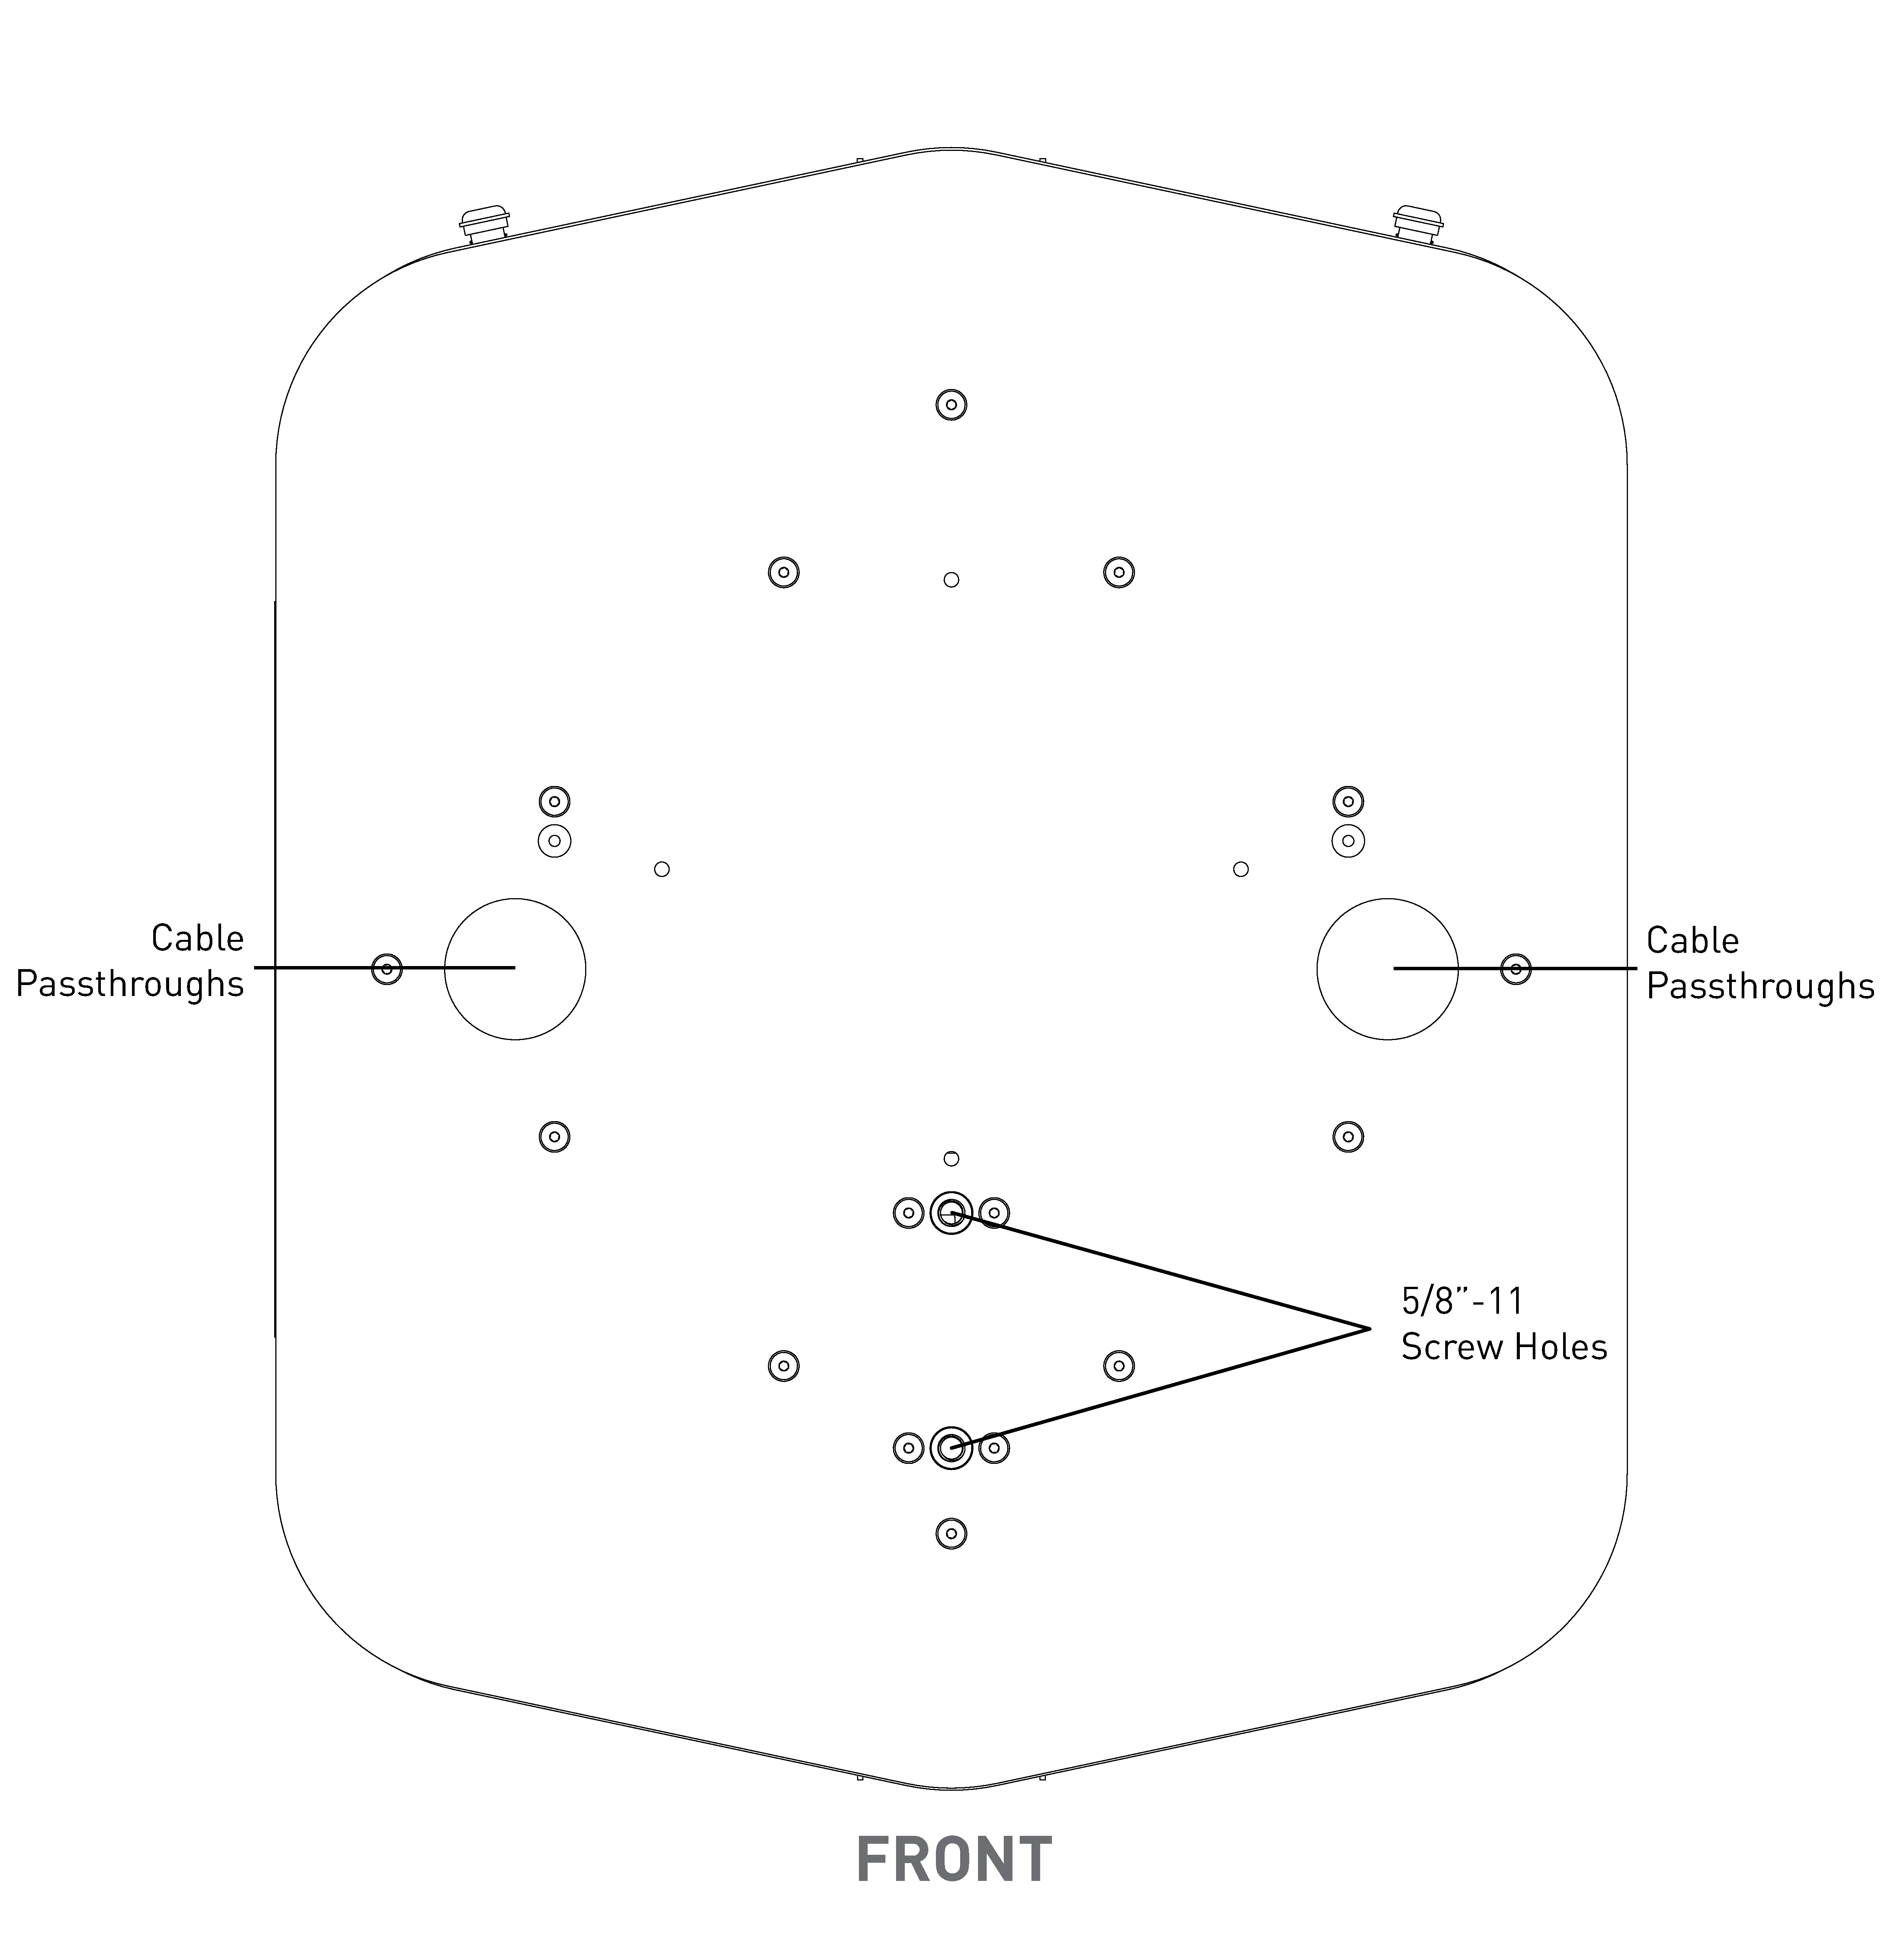
\includegraphics[width=0.75\linewidth]{Payload_Integration_Plate.pdf}
  \caption{Ridgeback Payload Integration}
  \label{payloadplate}
\end{figure}

\subsection{Electrical Integration}
\label{electrical}

The three white Molex user power receptacles located in the User Bay are capable of supplying 5Vdc, 12Vdc, and unregulated battery voltage (approximately 24Vdc) for powering Ridgeback's payloads. See the \autoref{userpower} for an labeled illustration and the pin assignments. The total draw allowed on each rail is 5-amps. The mating connector for these Molex Mini Fit Jr (tm) receptacles is 39-01-2040, available at Digikey (part number WM3701-ND.) Ensure you select the contact appropriate for the gauge of wire used. 

The single red and black Anderson connector pair provides unregulated battery voltage (approximately 24Vdc) at up to 20-amps peak. The mating parts are Anderson PP45 Power Pole (tm) 1327 (red housing), 1327G6 (black housing) and 261G2-LPBK (contacts.) These components are readily available at \url{Mouser.com}.

The rails on the User Bay Power board are protected against short circuit by fuses. See the illustration for the fuse locations and purposes. 

\textbf{WARNING:} For continued protection against risk of fire, always replace fuses only with those of the same type and rating.

\textbf{CAUTION:} The unregulated battery output may range from as low as 20Vdc up to 30Vdc or more depending on the state of charge of the battery pack and the electrical loading on the system. Ensure any accessories connected to that rail are able to deal with unregulated battery voltages.
  


\begin{figure}[h]
  \centering
  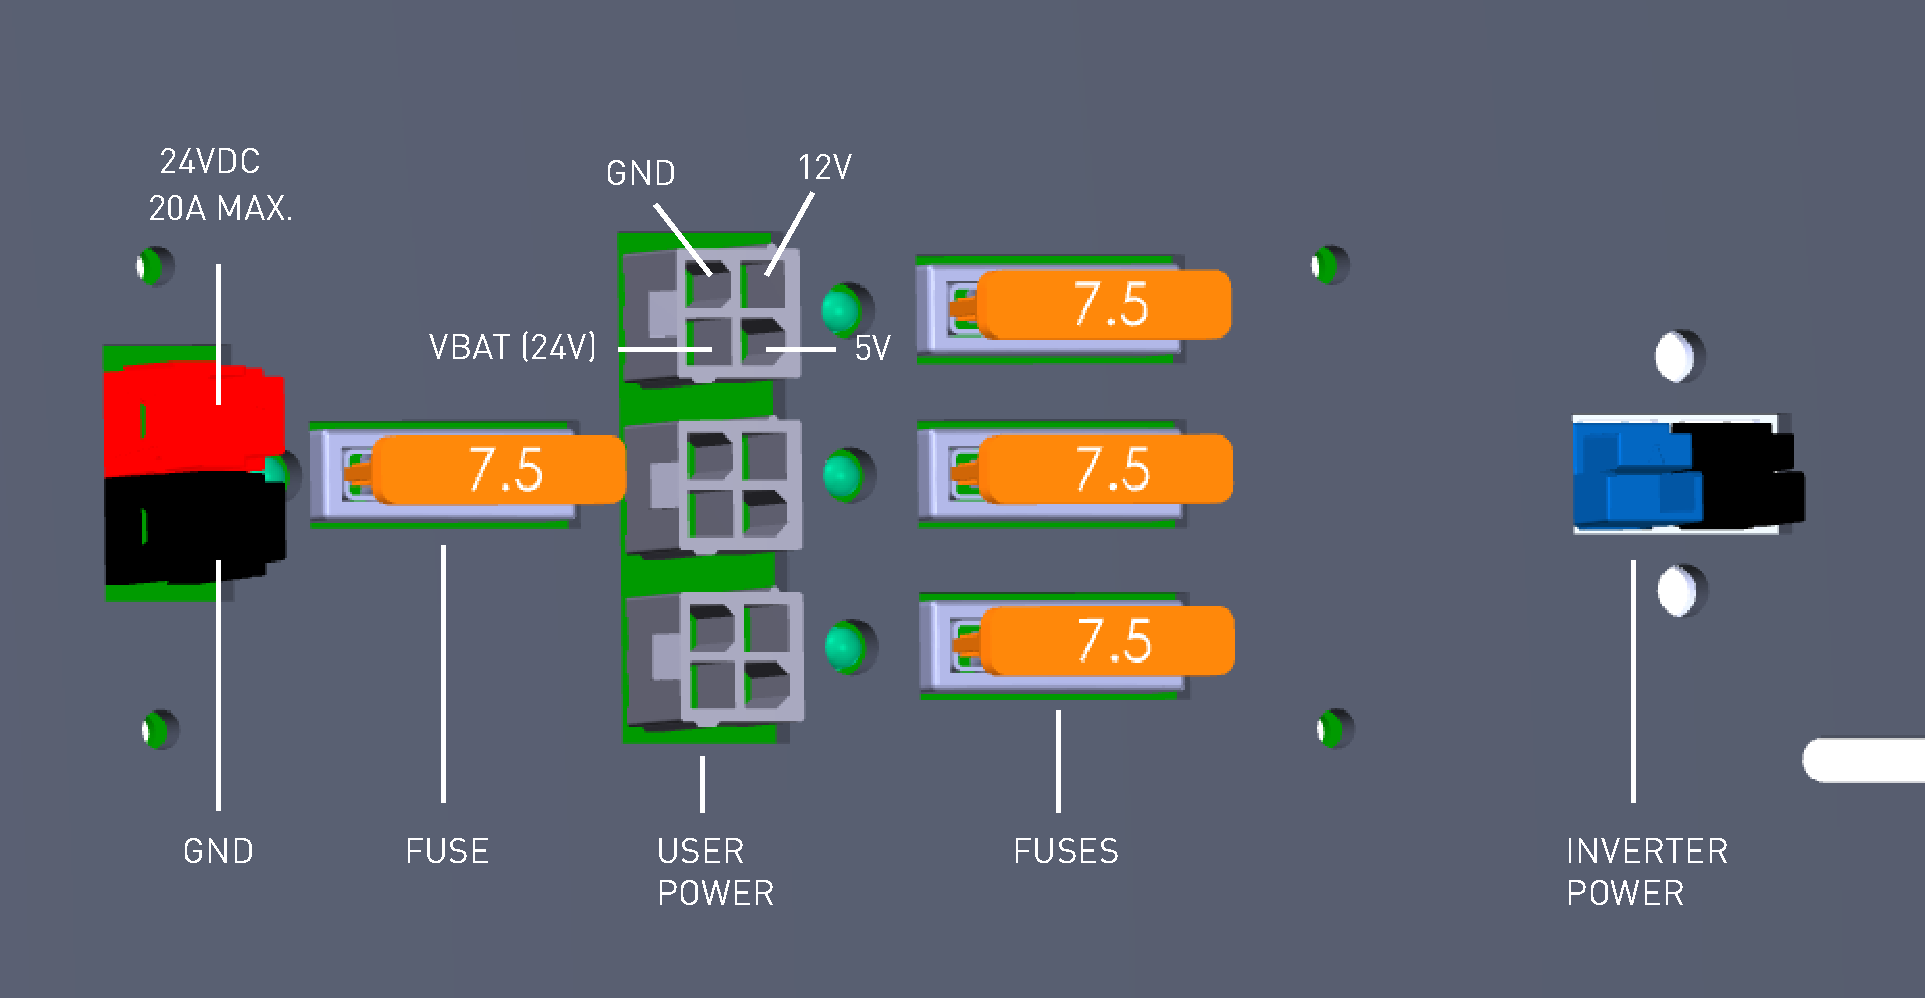
\includegraphics[width=1.0\linewidth]{Ridgeback_UserPower_SOLID.pdf}
  \caption{Ridgeback Power User Panel}
  \label{userpower}
\end{figure}





\subsection{Software Integration}

ROS has a large ecosystem of sensor drivers, some of which include pre-made URDF description and even simulation configurations.  Please see the following page on the ROS wiki for a partial list:

\url{http://wiki.ros.org/Sensors }

For the best experience, consider purchasing supported accessories from Clearpath Robotics for your Ridgeback, which will include simulation, visualization, and driver support.  However, we will happily assist you in integrating your own devices as well. 

\section{Maintenance}

\subsection{Battery Pack}

Refer to other section

\subsection{Fuses}

NEED CONTENT

\subsection{Tires}

NEED CONTENT

\subsection{Cleaning}

NEED CONTENT

\section{Contact}
\label{contact}

Clearpath is committed to your success with Ridgeback. Please get in touch with us and we’ll do our best to get
you rolling again quickly: \url{support@clearpathrobotics.com}.

To get in touch with a salesperson regarding Ridgeback or other Clearpath Robotics products, please email
sales@clearpathrobotics.com.

If you have a an issue that is specifically about ROS and is something which may be of interest to the broader
community, consider asking it on answers.ros.org. If you don’t get a satisfactory response, please ping us and
include a link to your question as posted there. If appropriate, we’ll answer in the ROS Answers context for
the benefit of the community.

Ridgeback is designed not to require regular maintenance. As it is a newer product, Clearpath appreciates your
patience as we understand its weak-point components and fill out the appropriate care instructions for the
platform.



\end{document}
